\documentclass[a4paper,12pt,titlepage]{article}
%\usepackage[T1]{fontenc}

\usepackage{titlesec}
\usepackage{titling}
\usepackage[portuguese]{babel}
\usepackage[utf8x]{inputenc}
\usepackage{indentfirst}
\usepackage{graphicx}
%\usepackage{times}
\usepackage{ucs}
\usepackage{float}    
\usepackage{fancyvrb}   
\usepackage{verbatim}
\usepackage{listings}
\usepackage{hyperref}
\usepackage{epigraph}
\usepackage{listings}
\usepackage{tabularx}
\usepackage{lipsum}
\usepackage{listings}
\usepackage{fancyvrb}   
\usepackage{verbatim}
\usepackage{listings}
\usepackage[usenames,dvipsnames]{xcolor}
\usepackage{caption}
\usepackage{hyperref}
\usepackage{epigraph}
\usepackage[raggedright]{sidecap}
\usepackage[nottoc,numbib]{tocbibind}
\usepackage{enumitem}

\hypersetup{
    colorlinks=true,       
    linkcolor=black,          
    citecolor=black,   
    filecolor=black,  
    urlcolor=black  
}

\hyphenation {di-re-cio-na-men-to} 

\captionsetup[figure]{width=10cm, font=small}
\captionsetup[SCfigure]{width=10cm, font=small}
\DeclareCaptionFont{white}{\color{white}}
\DeclareCaptionFormat{listing}{%
  \parbox{\textwidth}{\colorbox{gray}{\parbox{0.987\textwidth}{#1#2#3}}\vskip-4pt}}
\captionsetup[lstlisting]{format=listing,labelfont=white,textfont=white}
\lstset{frame=lrb,xleftmargin=1.15\fboxsep,xrightmargin=\fboxsep,language=[LaTeX]{TeX}}
\renewcommand{\lstlistingname}{Pseudo-código}
\lstloadlanguages{C++}
\lstset{%
  basicstyle=\ttfamily\color{black},
  commentstyle = \ttfamily\color{PineGreen},
  keywordstyle=\ttfamily\color{purple},
  stringstyle=\color{orange},
  numbers=left,
  numberstyle=\color{gray}}


%\renewcommand*{\familydefault}{\ttdefault}
\lstset{columns=fullflexible,basicstyle=\ttfamily}

\title{\large
Universidade Federal de Minas Gerais \\ \
Instituto de Ciências Exatas \\ \ 
Departamento de Ciência da Computação \\ \
\\[1cm]
Projeto e Análise de Algoritmos\\ \
3º Trabalho Prático - Paradigmas de Programação\\ \
\\[1cm]
\textbf{\Large A Spy History}
\\[1cm]
}

\author{\large Alberto Hideki Ueda \\[0.5cm] 
	Orientador: Berthier Ribeiro Neto 
\\[3cm] }

\date{\textsc{Belo Horizonte\\ \
14 de novembro de 2014}}

\begin{document}
\maketitle

\pagebreak

\section{Descrição do problema}

Dada um mensagem composta de \textit{bits} `0' e `1' e possíveis erros de transmissão, representados pelo símbolo `-', determinar se existe ou não um comando de controle na mensagem. Um erro de transmissão pode ser tanto um `0' quanto um `1'. Um comando de controle ou é uma sequência ``000" ou uma sequência ``11111". A resposta deve ser uma das seguintes:

\[
Resposta = 
\left \{
\begin{tabular}{lll}
$true$, se a mensagem com certeza contém um comando \\ de controle; \\
\\ 
$false$, se a mensagem com certeza não contém um \\ comando; \\
\\
$both$, se a mensagem pode ou não conter um comando,\\ dependendo do que os erros significarem. 
\end{tabular}
\right.
\]

\section{Modelagem}
% The description of the problem, how did you model it and how your algorithms work. The explanation of the algorithms must be clear, you can use pseudo-code for this.
A modelagem do problema é simples. Dada uma sequência de caracteres do conjunto $\{0, 1, -\}$ com tamanho máximo de 100 caracteres, determinar se tal sequência contém a subsequência ``000'' ou ``11111''; ou então se é possível substituir os caracteres `-' da sequência por \textit{bits} `0' e `1'  de forma que exista alguma destas subsequências. 

Há o caso particular em que mesmo que uma mensagem possua um ou mais caracteres `-', todas as formas de substituição possíveis contém subsequências de controle. Por exemplo, na mensagem ``1111-00'' todas as possíveis mensagens originais (``1111100'' e ``1111000'') contém um comando de controle. Neste e nos demais casos em que este cenário se aplica, naturalmente a resposta do algoritmo deve ser $true$.

Se há pelo menos uma possibilidade da mensagem não conter tais subsequências \textbf{E} pelo uma possibilidade dela conter, a resposta deve ser $both$.

Caso não haja nenhuma possibilidade da cadeia de caracteres conter um comando de controle, a resposta deve ser $false$. \ \\

A seguir serão descritos os três algoritmos propostos para lidar com o problema, cada um seguindo um paradigma de programação diferente.

\section{Algoritmo de Força Bruta}

\ \\ 
\begin{lstlisting}[caption=Algoritmo de Força Bruta]
string forca_bruta(string mensagem)
{
    se a mensagem for prevista em uma poda {
        determina a resposta com base na poda;
        devolve a resposta;
    } 
    senao {
        verifica_cada_mensagem_possivel(mensagem);
        devolve a resposta final obtida;
    }
}

string verifica_cada_mensagem_possivel(string mensagem);
{
    se existe caracter `-' na mensagem {
        verifica_cada_mensagem_possivel(mensagem_com_1);
        verifica_cada_mensagem_possivel(mensagem_com_0);
        combina as duas respostas e devolve uma unica;
    }
    senao {
        verifica se existe comando (mensagem);
        devolve resposta;
    }
}

\end{lstlisting}

\subsection{Complexidade de Espaço}
\subsection{Complexidade de Tempo}
\subsection{Análise Experimental}

\section{Algoritmo Guloso}

\begin{lstlisting}[caption=Algoritmo Guloso]
string guloso(string mensagem)
{
    para cada caracter do indice i da mensagem {
        se o caracter i = `-' {
            observa vizinhanca a esquerda e a direita;
            decide qual bit deve ser colocado no lugar de `-';
            verifica comando e guarda a resposta;
        } senao {
            verifica se existe um comando ate o caracter i;
            se existir o comando sem `-', devolve TRUE;
            se existir o comando com `-', guarda a resposta;
        }
        ++i;
    }
    
    se encontrou BOTH como resposta {
        devolve BOTH;
    } senao {
        devolve FALSE;
    }
}
\end{lstlisting}

\subsection{Complexidade de Espaço}
\subsection{Complexidade de Tempo}
\subsection{Análise Experimental}


\section{Algoritmo com Programação Dinâmica}
O algoritmo de PD adotado também utiliza a ideia de combinar respostas de subproblemas (algoritmo de força bruta). Mas desta vez são utilizados também dois contadores, um para 0s e outro para 1s. O sub-problema é encontrar a resposta para um determinado trecho da mensagem, dados os estados atuais de ambos os contadores. 

Cada resposta é armazenada em uma matriz de três dimensões ([índice do último caracter do trecho] $X$ [estado atual do contador de 1s] $X$ [estado atual do contador de 0s]).

Se for necessário resolver um sub-problema cuja resposta já esteja na matriz, basta consultar a resposta e utilizá-la. Caso a solução para este sub-problema ainda não tenha sido definida, o algoritmo realiza o cálculo de tal resposta com base nos resultados de outros sub-problemas. \ \\

Sejam: 
\begin{itemize}[leftmargin=1.5cm]
    \item mensagem: a instância do problema;
    \item n: tamanho da mensagem;
    \item i : índice do caracter que está sendo analisado. A sub-mensagem [0..i-1] já foi analisada;
    \item c1 : contador de 1's;
    \item c0 : contador de 0's;
    \item opt : a resposta para o subproblema de acordo com os parâmetros. Um dos valores do conjunto $\{true, false, both\}$.
    \ \\
\end{itemize}

A função de recorrência utilizada é a seguinte: 
\ \\

\[ 
opt (i, c1, c0) = 
\left \{
\begin{tabular}{lll}
// condições de parada \\
$true$, se c1 = 5 ou se c0 = 3; \\
$false$, se i = n; \\
\\ 
// recursão. Casos `1' ou `0'\\
$opt$ (i, c1+1, 0) , se mensagem[i] = `1'; \\
$opt$ (i, 0, c0+1) , se mensagem[i] = `0'; \\
\\
// recursão. Caso `-'\\
$both$, se $opt$ (i, c1+1, 0) != $opt$ (i, 0, c0+1);\\
$opt$ (i, 0, c0+1), caso contrário.\\
\end{tabular}
\right.
\]

\subsection{Complexidade de Espaço}
\subsection{Complexidade de Tempo}
\subsection{Análise Experimental}


\section{Dificuldades Encontradas}

Algumas das principais dificuldades encontras neste trabalho prático foram: 
\begin{itemize}[leftmargin=1.5cm]
    \item Discernimento entre os três paradigmas ao analisar ideias para os algoritmos. Não foi raro descobrir que ideias para um algoritmo de determinado paradigma eram na realidade de outro paradigma. Por exemplo, percorrer trechos de uma mensagem e testar todas as possibilidades é uma estratégia que pode ser vista como gulosa em um primeiro momento, apesar de ser na realidade de força bruta.
    \item Algoritmo de Programação Dinâmica: o resultado apresentando neste trabalho foi construído após muitas discussões e colaboração de colegas do departamento de computação. Muitas tentativas anteriores não tiveram sucesso ou foram descartadas ao decorrer do trabalho;
    \item Hipótese incorreta das possibilidades de $true$. A princípio, acreditávamos que apenas `00-1111' e '1111-00' eram as mensagens que, apesar de conter incertezas, tinham como resposta correta $true$. Porém, mais tarde descobrimos outros casos, como por exemplo: `00-111-00' e `00-111-0-1111'. Essa foi uma das descobertas que desmotivou a busca de um algoritmo ótimo no caso do guloso.
    \ \\
\end{itemize}


\section{Conclusão}
% A brief conclusion of the work
Este trabalho prático foi bastante útil para fixar o aprendizado do módulo de paradigmas de programação. Lidar com problemas práticos exigiu um bom (re)estudo do conteúdo teórico. Outro ponto a destacar foi constatação que um algoritmo de força-bruta não é necessariamente mais simples de implementar que um algoritmo guloso, por exemplo. A percepção de que muitas vezes um algoritmo que ``testa todos os casos" pode e deve ser melhorado significamente pode sutilmente ocultar o esforço e o valor de um algoritmo de força-bruta. O conceito de $poda$ também ficou muito mais claro com este trabalho prático.

A descoberta de que o problema pode ser solucionado por um algoritmo de complexidade de tempo linear foi surpreendente. O algoritmo de programação dinâmica, apesar de utilizar mais espaço para sua execução, é muito mais veloz que o algoritmo guloso e naturalmente que o de força-bruta também. Graças à divisão do problema original em subproblemas que se repetem e que podem ter a resposta memoizada, o desepenho de tal algoritmo mostrou resultados bastante satisfatórios e por si só justifica o estudo e pesquisa empreendidos nesta área de conhecimento.

\begin{figure}[H]
     \centering
     % 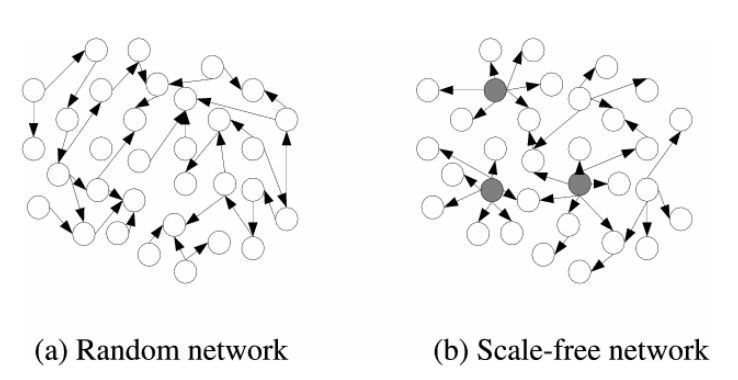
\includegraphics[scale=0.5]{figures/network-types.png}
     \caption{}
     \label{bsp}
\end{figure}


% Referências
\bibliographystyle{plain}%amsalpha
\bibliography{bibliografia}
\newpage

\end{document}


